\subsection{Tipo de entidad Pregunta}

   \begin{description}

   \item[Definición] Se refiere al objeto del mundo real: \emph{``Cuestión planteada por el usuario asesor al usuario alumno''}.

   \item[Características] La entidad presenta las siguientes características:
      \begin{itemize}
         \item \textbf{Nombre:} Pregunta.
         \item \textbf{Tipo:} Débil por identificación con respecto a Entrevista.
         \item \textbf{Número de atributos:} 2 propios y 1 heredado.
         \item \textbf{Atributo/s identificador/es principal/es:} id\_entrevista
         junto con el atributo id\_pregunta.
         \item \textbf{Atributo/s identificador/es alternativo/s:} -
         \item \textbf{Atributo/s heredado/s:} id\_entrevista del tipo de
         entidad Entrevista.
      \end{itemize}

   \item[Diagrama] La figura \ref{diagramaPregunta} muestra el diagrama de la entidad.
   \item \begin{figure}[!ht]
            \begin{center}
            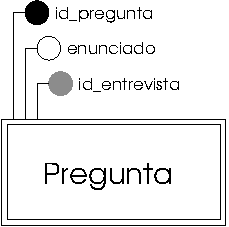
\includegraphics[]{07.Modelo_Entidad-Interrelacion/7.2.Analisis_Entidades/diagramas/pregunta.pdf}
            \caption{Diagrama de la entidad Pregunta.}
            \label{diagramaPregunta}
            \end{center}
         \end{figure}

   \item[Descripción de los atributos propios] La entidad presenta los siguientes
   atributos propios:

   \begin{itemize}
    \item \textbf{id\_pregunta}
      \begin{itemize}
         \item \textbf{Definición:} Código que sirve como número identificativo
               para cada pregunta del sistema.
         \item \textbf{Dominio:} Números naturales.
         \item \textbf{Carácter:} Obligatorio.
         \item \textbf{Ejemplo práctico:} 36.
         \item \textbf{Información adicional:} El dato lo genera el sistema
               cuando se introduce una nueva pregunta en el sistema. Es la clave
               primaria.
      \end{itemize}
   \item \textbf{enunciado}
      \begin{itemize}
         \item \textbf{Definición:} Cuestión planteada por el asesor al alumno.
         \item \textbf{Dominio:} Conjunto de caracteres alfanuméricos.
         \item \textbf{Carácter:} Obligatorio.
         \item \textbf{Ejemplo práctico:} Nivel de inglés.
         \item \textbf{Información adicional:} El dato lo introduce el
         administrador principal al introducir una nueva pregunta en el sistema.
      \end{itemize}
   \end{itemize}

   \item[Ejemplo práctico]

   \item \begin{center}
            \begin{tabular}{ | l | l | }
            \hline
            \multicolumn{2}{ | c | }{\textbf{Tipo de entidad Pregunta}} \\
            \hline
            id\_pregunta & 36 \\
            \hline
            enunciado & Nivel de inglés \\
            \hline
            id\_entrevista & 24 \\
            \hline
            \end{tabular}
         \end{center}
   \end{description}
